%% This is an example first chapter.  You should put chapter/appendix that you
%% write into a separate file, and add a line \include{yourfilename} to
%% main.tex, where `yourfilename.tex' is the name of the chapter/appendix file.
%% You can process specific files by typing their names in at the 
%% \files=
%% prompt when you run the file main.tex through LaTeX.
\chapter{Results}

\section{Perturation of States}

Early attempts at running the DSHKEnKF on the hydrologic model were marked by the complete collapse of posterior ensemble covariance to the mean and erratic jumps from the minimum to the maximum bounds for all streamflow parameters. Snow water equivalent parameters and states, however, converged in a stable fashion. It was determined that these erratic jumps were due to the hydrologic model's dependence on the value of the catchments' lowest groundwater reservoir, an unobserved and uncorrected state, which was integral to the production of streamflow in each timestep. White noise added to the forcing data (precipitation and min/max temperature) was unable to generate adequately diverse ensemble behavior when groundwater states were uniform across ensembles. To account for this, perturbation of groundwater and streamflow states was implemented.

\subsection{Perturbation of Groundwater States}

The hydrologic model was extremely sensitive to its starting states, in particular the lower groundwater reservoir. A low groundwater would lead to underwhelming groundwater, incentivising the parameters \textit{ck0}, \textit{ck1}, and \textit{ck2} to converge towards values that emptied all water pouring into the reservoirs so modeled streamflow could match the observations. Conversely, high starting groundwater caused \textit{ck0}, \textit{ck1}, and \textit{ck2} to converge towards parameters that let very little groundwater out of the reservoirs, further exasperating the problem and causing higher and higher values for \textit{ck0}, \textit{ck1}, and \textit{ck2} to be chosen. 

To solve this issue and find a reliable blanket starting value for groundwater subcatchments in an efficient amount of time the small dataset was utilized alongside the parameter boundaries specified by \cite{Maneta2008}. Trial and error was utilized on the dataset until groundwater stabilized. To encourage the model to explore different parameter values for different amounts of groundwater, initial states for the large dataset were perturbed across all ensembles and catchments using a $\mu$ equal to the average stable value of the small dataset, which for this model was roughly calculated to be 100mm, and a $\sigma$ of 80mm. During the prediction phase groundwater was treated as forcing data and was perturbed slightly at a $\sigma$ of $u_{gw} * gw$, with $u_{gw}$  at .05%.

\begin{figure}
\centering
\begin{minipage}{.5\textwidth}
  \centering
  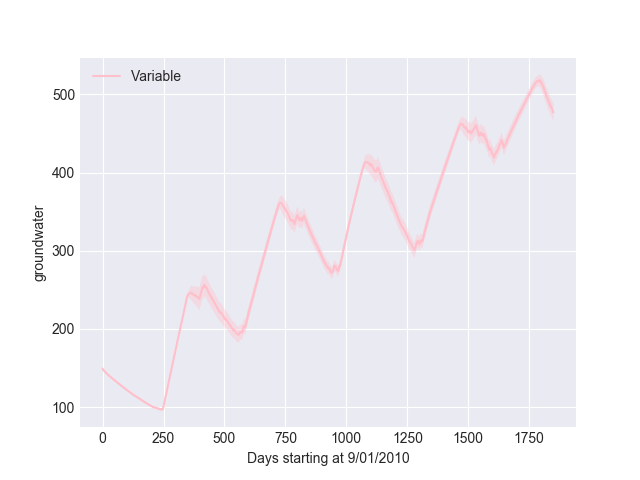
\includegraphics[width=.98\linewidth]{bad_gw}
  \captionof{figure}{Uniform groundwater}
  \label{fig:bad_gw}
\end{minipage}%
\begin{minipage}{.5\textwidth}
  \centering
  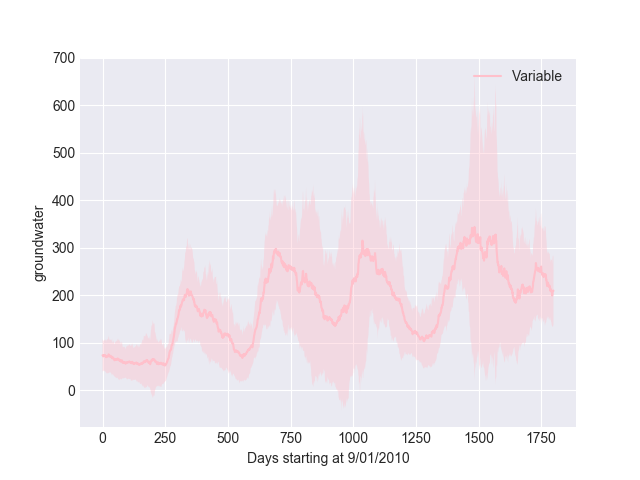
\includegraphics[width=.94\linewidth]{good_gw}
  \captionof{figure}{Perturbed groundwater}
  \label{fig:good_gw}
\end{minipage}
\end{figure}


\subsection{Continuous perturbation of streamflow and swe states}

Another method of decoupling the model's calibration process from its over-reliance on groundwater was through the direct perturbation of streamflow and swe states. This perturbation guaranteed that ensemble collapse was never fully realized.


\section{Small dataset}

The small dataset, comprised of 3 catchments around the Biterroot valley, converged to a series of parameters very quickly. The small dataset was run over a period of 1800 days, or a little under 5 years. The simulation began in September so modeled snowfall accumulation could be corrected first, allowing accurate snowmelts to inform streamflow runoff in the Spring and Summer. 


\begin{table}[]
\caption{Hyperparameters - parameter perturbations and min/max ranges} 
\begin{tabular}{llll}
Parameter ($\theta$) & $q$ & Min & Max \\ \hline
Degree Day Factor (\textit{ddf})                 & .75mm$^\circ$C$^{-1}$d$^{-1}$ & 1mm$^\circ$C$^{-1}$d$^{-1}$ & 8mm$^\circ$C$^{-1}$d$^{-1}$ \\
Tempature Threshold (\textit{thres})                & .5$^\circ$C & -2.5$^\circ$C & 2.5$^\circ$C \\
Potential Evapo-Transpiration (\textit{aet\_lp})              & .15 & .3 & 1\\
Ponded water to soil storage (\textit{soil\_beta})          & 1.75 & 1 & 6 \\
Soil compartment max capacity (\textit{soil\_max\_wat})       & 40 & 50mm & 500mm \\
Immediate runoff (\textit{ck0})       & 6d$^{-1}$ & .25d$^{-1}$ & 10d$^{-1}$ \\
Fast runoff (\textit{ck1})      & 25d$^{-1}$ & 3.33d$^{-1}$ & 50d$^{-1}$\\
Groundwater runoff (\textit{ck2})       & 350d$^{-1}$ & 50d$^{-1}$ & 650d$^{-1}$ \\
Groundwater water storage threshold (\textit{hl1})       & 25mm & 0mm & 50mm \\
Groundwater peculation (\textit{perc})       & 1.5d & 3d & 50d \\
Wave celerity (\textit{K})         & 82400 & 81576 & 84872 \\
Wave dispersion (\textit{e})       & .35 & .25 & .4 \\
\end{tabular}
\label{tab:t_param_min_max}
\end{table}

